\chapter{Team 2 Agent Design}\label{team_2_agent_design}\chapter{Team 2 Agent Design}\label{team_2_agent_design}

\section{Overview}
(To do)

\section{Action decision}
When the agent has to make its own decision, the \verb|FightAction(...)| function is called and returns the decision. Its basic process is illustrated in \autoref{fig:fightaction}.

\begin{figure}[h!]
    \centering
    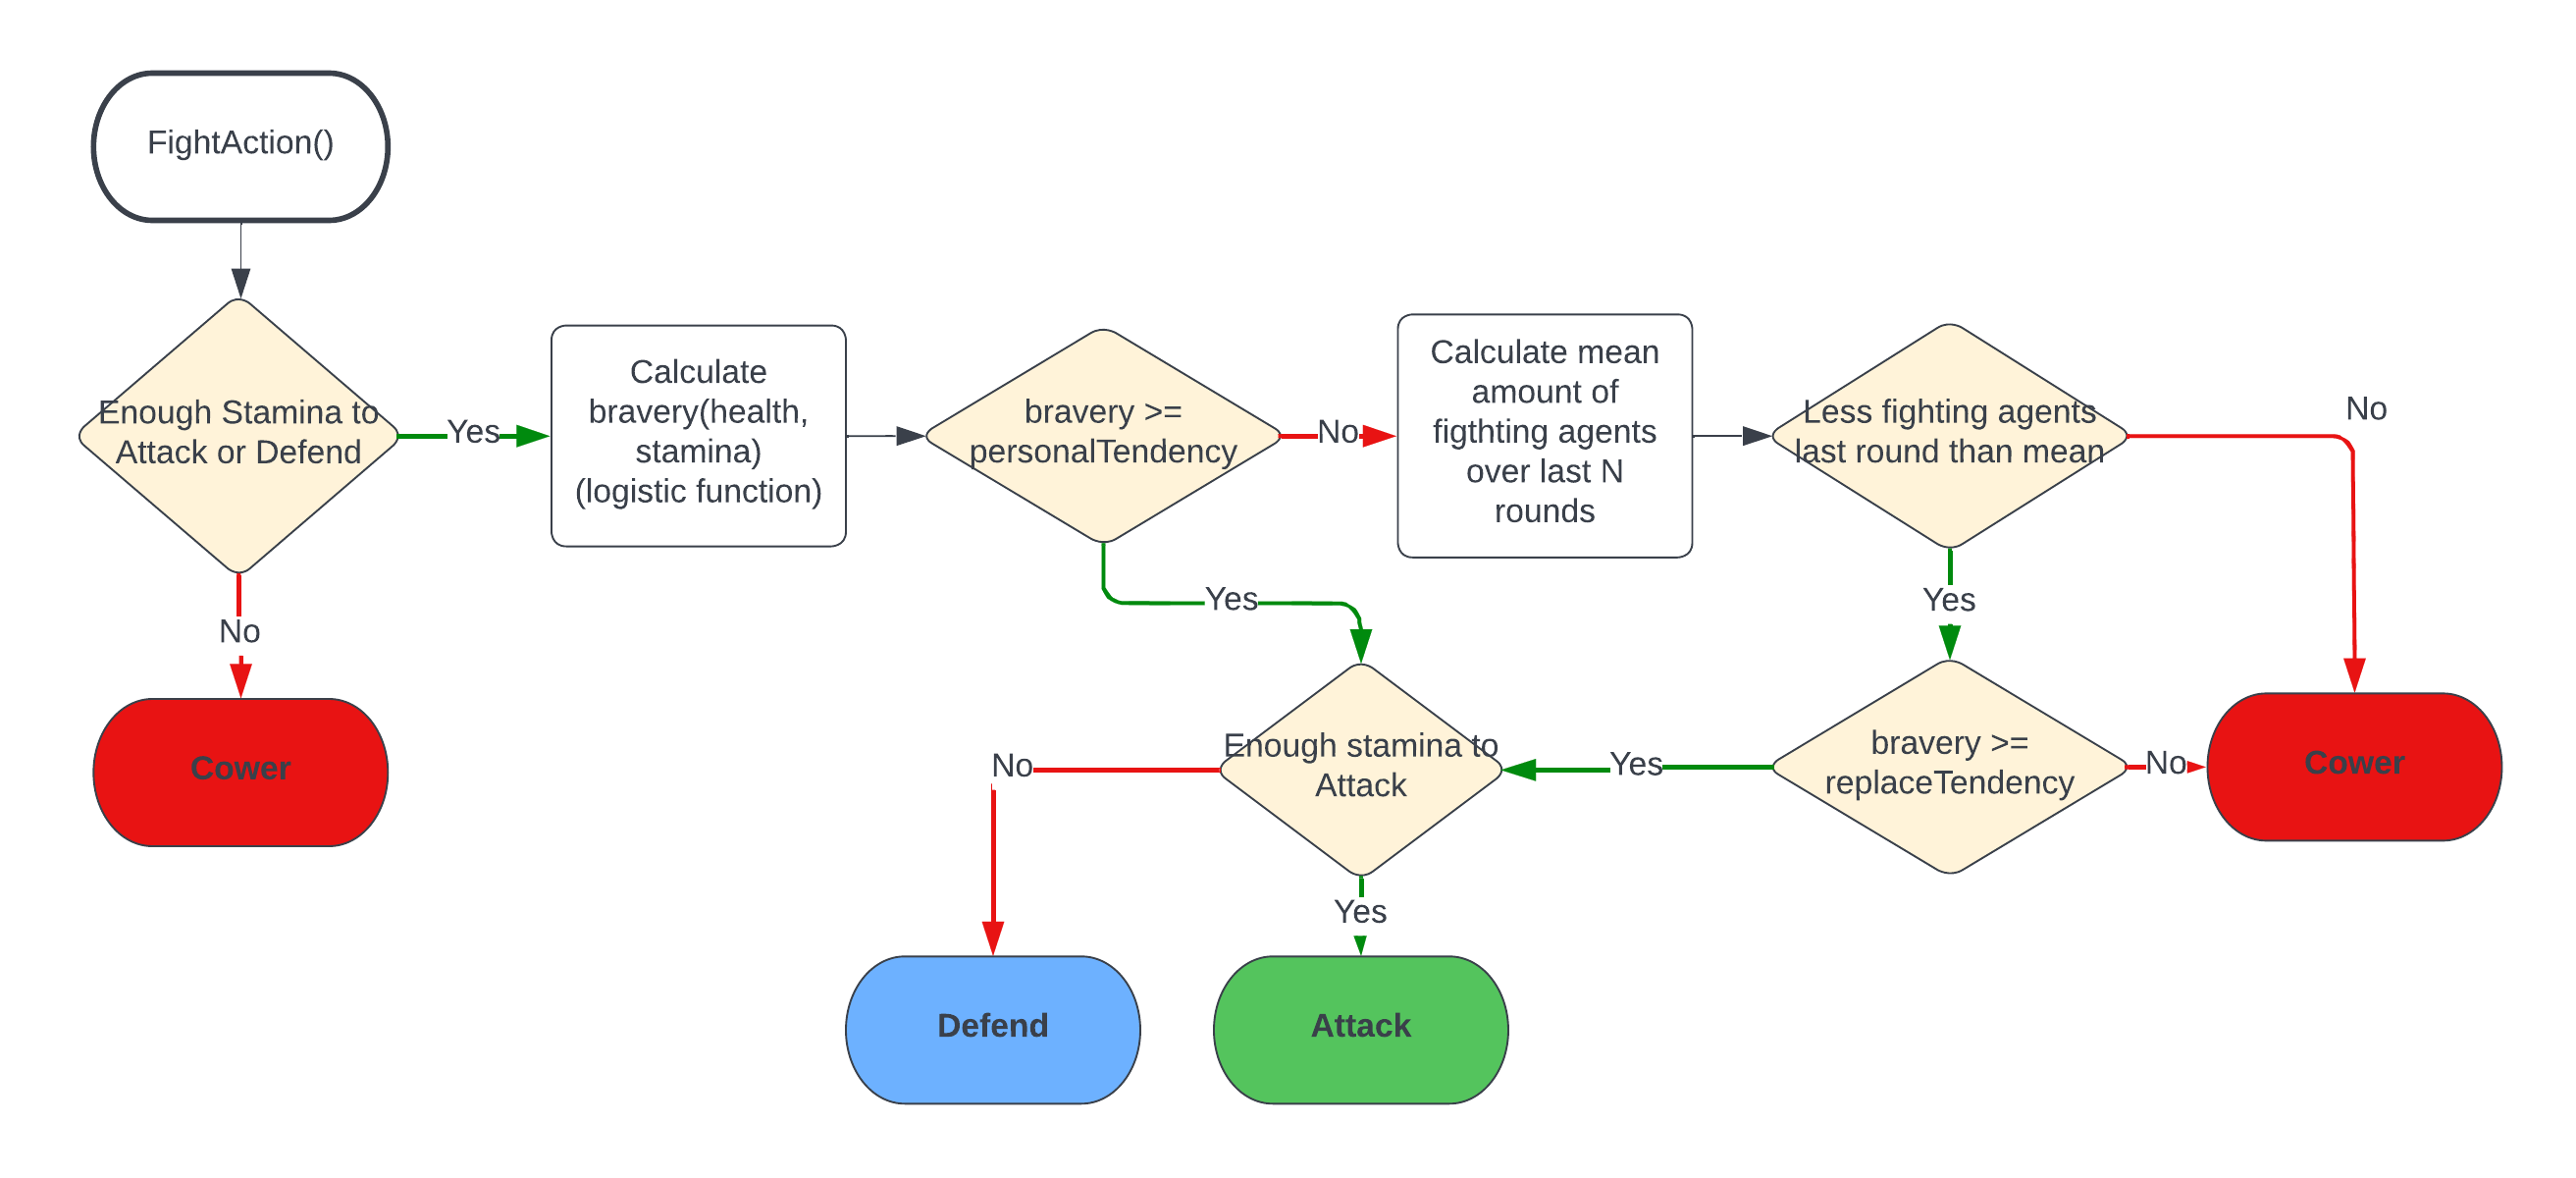
\includegraphics[width=\linewidth]{SOMAS-Agent2-Report/fightaction.png}
    \caption{Process of personal decision making}
    \label{fig:fightaction}
\end{figure}

Each agent contains two character traits, generated at the program's initialisation : \begin{itemize}
    \item \verb|personalTendency| $\in[0,1]$ : the agent's tendency to fight
    \item \verb|replaceTendency| $\in[0,1]$ : the agent's tendency to replace non-fighting agents
\end{itemize}
Additionally, each time \verb|FightAction()| is called, a fluent variable \verb|bravery| is computed such as $$\verb|bravery|(\verb|health|, \verb|stamina|) = \frac{0.5}{1+e^{-0.01(health-500)}} + \frac{0.5}{1+e^{-0.005(stamina-1000)}}$$
which is a combination of two spread logistic functions over the range of \verb|health| and \verb|stamina|.

 \verb|bravery|, $\in [0,1]$, represents the current "confidence"\footnote{The variable bravery was not named confidence in order to avoid mistaking it with the confidence in the leader.} an agent has depending on its state : the more health and stamina it has, the braver it feels.

 \paragraph{Initial decision}

 By comparing its current \verb|bravery| to its \verb|personalTendency|, the first makes a decision to act or cower. If $\verb|bravery| > \verb|personalTendency|$, it will end the function and return either Attack or Defend. If not, it will first decide to cower.


 \paragraph{Replacement decision}

 If the answer to the initial decision was Cower, the agent will then use the history mechanism (its memory) to observe the overall trend in decisions. It computes the mean of fighting/defending agents over the last $N$ rounds, and if it find that last round was lower than the mean, it will reconsider its decision.

 Then, if  $\verb|bravery| > \verb|replaceTendency|$, it will either Attack or Defend. Else, it will stay in a cowering state.

\paragraph{Not-implemented : damage estimation}

This part was not implemented because at some point, it was decided on the infrastructure side that agents would not have access to the entire set of current agents decisions, and that peer-to-peer communication would be limited.

An additional test was supposed to be made, where the agent would try to estimate the current damage and defense based on the current set of decision, and possibly decide to act if it found these values to be too low. The decision would have followed the same process as before.

\subsection{Behaviour}
Overall, with the right parameters, the agents will try to act as much as they can while preserving their own health. They will occasionally override their own decision for the greater good, to try to replace cowering agents.


\section{Manifesto}

Influenced by the concept of relevant expertise aggregation, we thought that we could treat our agent as an "expert singleton" as far as leadership candidacy is concerned. We decided that we will be quantifying our expertise in order to be able to derive what values we could reasonably set in our 'manifesto' i.e. the terms of leadership we put forward in any election. This quantification metric, which can be also thought as an equivalent indicator of credibility in a trust framework, was set as follows:(Explanation of 2 eq). 

Through \verb|ManifestoEffectiveness| we can measure how well we perform when we request a fight decision or loot imposition. It should also be highlighted that expertise does not always increase, but instead it can decrease as well (so it is different to the concept of experience). In order to derive the term length, we map our expertise to a range between 0 and 4 and add it to a default value of 1. In other words, in the very beginning, if we don't have any expertise at all, we request a term length of 1, (which is reasonable due to our lack of expertise), but as we start to gain expertise the term length will dynamically adjust in the range [1,5]. Moving on to fight decision power, we wanted to be able to take into consideration the previous leaders' manifestos and whether they were deposed, since we thought that perhaps the cohort would not trust a new leader with the same manifesto as a previous leader who was deposed. More specifically, we start by checking whether the previous leader had fight decision power and whether he was deposed. If both are true, we take our expertise and subtract from it a small negative bias. Then, if this total value is greater than a threshold, we set \verb|fightDecisionPower| to true in our manifesto. An equivalent logic has been implemented for determining whether \verb|lootDecisionPower| should be true. Finally, for deriving the no-confidence percentage required for our leader to get deposed, we map our expertise to a range of [-10\%, 10\%] and add this value to a default percentage of 51\%, considering that if we do not have any expertise, a simple majority of 51\% would be a reasonable value, but as we start having more expertise, that value should be dynamic and within the range [41\%,61\%], since a more 'expert' leader is more credible and trustworthy, therefore shouldn't be as easy to depose (and vice versa for a less expert leader).\\

\section{Fight strategy} If this agent is elected as a leader, we will have the following fighting strategy: we will propose that agents with Health lower than the bare minimum should Cower, thus forcing those who are the most vulnerable to survive and regenerate health; agents with Health greater than the baseline and attack and defend greater than the minimum required will be suggested to attack and defend as it is their moral obligation to perform these actions and lead the fight; remaining agents that do not fall within these parameters will be free to perform their own Actions. We will choose to broadcast the proposals of other agents with a similar strategy (?). Elasticity will be used to allow a range for Minimum and Baseline values to be checked with the Proposal if they are satisfied.(Explain Elasticity?)\\

\section{No-confidence vote}
To handle the no-confidence vote for the leader, at the end of each level, we implement a generic social capital framework. More specifically, we takes as 'events' information about the game yielded under that agent's leadership - such as remaining agents after each round/level, fighting statistics for the leader etc. Then, we use 'event handler' functions to convert these to useful quantitative metrics - such as how many (if any) times they were a leader before, if they were voted out in on-confidence, the rate at which the agent pool is decreasing, how frequently agents are given the floor for proposals etc.(...). These metrics are in turn normalized with respect to their global averages (otherwise their magnitudes are meaningless; normalizing gives an indication of how much better or worse the leader is performing compared to other leaders). Then, these are selectively weighted and summed to yield social capital values for the current leader. Namely, 'trustworthiness' is measured as how positively their leadership impacts the collective, through combining the survival rates under their current and previous leaderships (weighting the former more). 'Networks' are (tenuously...) measured as the rate, again from both current and previous leaderships, at which the leader broadcasts proposals our agent has submitted to them. This sort of quantifies how communicative the leader is. Finally, 'Institution' is measured as a combicnation and how successfully they wielded it

\\

\section{Election of a leader}To select a preference for the leader, we again take into consideration two of the metrics used in the social capital framework, but only the two values, but also the manifesto of the prospect leaders. More specifically, to vote for a leader we compute a score for each prospect leader, based on the following parameters. If the leader requires a fight imposition, we add a small negative bias to the score of the prospect leader. This is, because especially if the leader has not been elected before and has no expertise, we prefer that he does not impose(/ propose?) a fight. We rather want that this decision comes from all the agents collectively. Equivalently, we add a small negative bias if the leader requires a loot imposition. Additionally,another parameter that we take into account is the Sot(overthrow percentage+term length). We sum the overthrow percentage and term length for each prospect leader and then rank them in descending order (the one with the smallest overthrow percentage+term length gets the highest points). Now, if the leader has been elected before, we also consider the two social capital parameters mentioned before. Finally,we weigh these parameters, we sum them and we vote for the agent with the highest score. The highest weights are given to the parameters associated with past leadership data, because we think that expertise is crucial for a leader.\\

\section{Weapon and shield selection}Additionally, considering that our agent can only attack or defend if our stamina is greater than our BonusAttack, we decided that whenever we choose to fight, we should fight with the weapon with the highest BonusAttack given our Stamina at that point. Equivalently, our agent always chooses the Shield with the highest BonusDeafence.\\

\section{HP pool donation}In terms of HP(Health Points), our agent always donates to the common pool if his health points our greater than a threshold. The amount of health points given at the end of each level is dynamically adjusted according to: (explain math formula).

